\documentclass[1p]{elsarticle_modified}
%\bibliographystyle{elsarticle-num}

%\usepackage[colorlinks]{hyperref}
%\usepackage{abbrmath_seonhwa} %\Abb, \Ascr, \Acal ,\Abf, \Afrak
\usepackage{amsfonts}
\usepackage{amssymb}
\usepackage{amsmath}
\usepackage{amsthm}
\usepackage{scalefnt}
\usepackage{amsbsy}
\usepackage{kotex}
\usepackage{caption}
\usepackage{subfig}
\usepackage{color}
\usepackage{graphicx}
\usepackage{xcolor} %% white, black, red, green, blue, cyan, magenta, yellow
\usepackage{float}
\usepackage{setspace}
\usepackage{hyperref}

\usepackage{tikz}
\usetikzlibrary{arrows}

\usepackage{multirow}
\usepackage{array} % fixed length table
\usepackage{hhline}

%%%%%%%%%%%%%%%%%%%%%
\makeatletter
\renewcommand*\env@matrix[1][\arraystretch]{%
	\edef\arraystretch{#1}%
	\hskip -\arraycolsep
	\let\@ifnextchar\new@ifnextchar
	\array{*\c@MaxMatrixCols c}}
\makeatother %https://tex.stackexchange.com/questions/14071/how-can-i-increase-the-line-spacing-in-a-matrix
%%%%%%%%%%%%%%%

\usepackage[normalem]{ulem}

\newcommand{\msout}[1]{\ifmmode\text{\sout{\ensuremath{#1}}}\else\sout{#1}\fi}
%SOURCE: \msout is \stkout macro in https://tex.stackexchange.com/questions/20609/strikeout-in-math-mode

\newcommand{\cancel}[1]{
	\ifmmode
	{\color{red}\msout{#1}}
	\else
	{\color{red}\sout{#1}}
	\fi
}

\newcommand{\add}[1]{
	{\color{blue}\uwave{#1}}
}

\newcommand{\replace}[2]{
	\ifmmode
	{\color{red}\msout{#1}}{\color{blue}\uwave{#2}}
	\else
	{\color{red}\sout{#1}}{\color{blue}\uwave{#2}}
	\fi
}

\newcommand{\Sol}{\mathcal{S}} %segment
\newcommand{\D}{D} %diagram
\newcommand{\A}{\mathcal{A}} %arc


%%%%%%%%%%%%%%%%%%%%%%%%%%%%%5 test

\def\sl{\operatorname{\textup{SL}}(2,\Cbb)}
\def\psl{\operatorname{\textup{PSL}}(2,\Cbb)}
\def\quan{\mkern 1mu \triangleright \mkern 1mu}

\theoremstyle{definition}
\newtheorem{thm}{Theorem}[section]
\newtheorem{prop}[thm]{Proposition}
\newtheorem{lem}[thm]{Lemma}
\newtheorem{ques}[thm]{Question}
\newtheorem{cor}[thm]{Corollary}
\newtheorem{defn}[thm]{Definition}
\newtheorem{exam}[thm]{Example}
\newtheorem{rmk}[thm]{Remark}
\newtheorem{alg}[thm]{Algorithm}

\newcommand{\I}{\sqrt{-1}}
\begin{document}

%\begin{frontmatter}
%
%\title{Boundary parabolic representations of knots up to 8 crossings}
%
%%% Group authors per affiliation:
%\author{Yunhi Cho} 
%\address{Department of Mathematics, University of Seoul, Seoul, Korea}
%\ead{yhcho@uos.ac.kr}
%
%
%\author{Seonhwa Kim} %\fnref{s_kim}}
%\address{Center for Geometry and Physics, Institute for Basic Science, Pohang, 37673, Korea}
%\ead{ryeona17@ibs.re.kr}
%
%\author{Hyuk Kim}
%\address{Department of Mathematical Sciences, Seoul National University, Seoul 08826, Korea}
%\ead{hyukkim@snu.ac.kr}
%
%\author{Seokbeom Yoon}
%\address{Department of Mathematical Sciences, Seoul National University, Seoul, 08826,  Korea}
%\ead{sbyoon15@snu.ac.kr}
%
%\begin{abstract}
%We find all boundary parabolic representation of knots up to 8 crossings.
%
%\end{abstract}
%\begin{keyword}
%    \MSC[2010] 57M25 
%\end{keyword}
%
%\end{frontmatter}

%\linenumbers
%\tableofcontents
%
\newcommand\colored[1]{\textcolor{white}{\rule[-0.35ex]{0.8em}{1.4ex}}\kern-0.8em\color{red} #1}%
%\newcommand\colored[1]{\textcolor{white}{ #1}\kern-2.17ex	\textcolor{white}{ #1}\kern-1.81ex	\textcolor{white}{ #1}\kern-2.15ex\color{red}#1	}

{\Large $\underline{12a_{0047}~(K12a_{0047})}$}

\setlength{\tabcolsep}{10pt}
\renewcommand{\arraystretch}{1.6}
\vspace{1cm}\begin{tabular}{m{100pt}>{\centering\arraybackslash}m{274pt}}
\multirow{5}{120pt}{
	\centering
	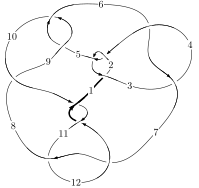
\includegraphics[width=112pt]{../../../GIT/diagram.site/Diagrams/png/848_12a_0047.png}\\
\ \ \ A knot diagram\footnotemark}&
\allowdisplaybreaks
\textbf{Linearized knot diagam} \\
\cline{2-2}
 &
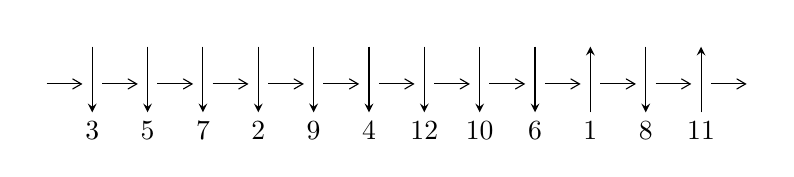
\begin{tikzpicture}[x=20pt, y=17pt]
	% nodes
	\node (C0) at (0, 0) {};
	\node (C1) at (1, 0) {};
	\node (C1U) at (1, +1) {};
	\node (C1D) at (1, -1) {3};

	\node (C2) at (2, 0) {};
	\node (C2U) at (2, +1) {};
	\node (C2D) at (2, -1) {5};

	\node (C3) at (3, 0) {};
	\node (C3U) at (3, +1) {};
	\node (C3D) at (3, -1) {7};

	\node (C4) at (4, 0) {};
	\node (C4U) at (4, +1) {};
	\node (C4D) at (4, -1) {2};

	\node (C5) at (5, 0) {};
	\node (C5U) at (5, +1) {};
	\node (C5D) at (5, -1) {9};

	\node (C6) at (6, 0) {};
	\node (C6U) at (6, +1) {};
	\node (C6D) at (6, -1) {4};

	\node (C7) at (7, 0) {};
	\node (C7U) at (7, +1) {};
	\node (C7D) at (7, -1) {12};

	\node (C8) at (8, 0) {};
	\node (C8U) at (8, +1) {};
	\node (C8D) at (8, -1) {10};

	\node (C9) at (9, 0) {};
	\node (C9U) at (9, +1) {};
	\node (C9D) at (9, -1) {6};

	\node (C10) at (10, 0) {};
	\node (C10U) at (10, +1) {};
	\node (C10D) at (10, -1) {1};

	\node (C11) at (11, 0) {};
	\node (C11U) at (11, +1) {};
	\node (C11D) at (11, -1) {8};

	\node (C12) at (12, 0) {};
	\node (C12U) at (12, +1) {};
	\node (C12D) at (12, -1) {11};
	\node (C13) at (13, 0) {};

	% arrows
	\draw[->,>={angle 60}]
	(C0) edge (C1) (C1) edge (C2) (C2) edge (C3) (C3) edge (C4) (C4) edge (C5) (C5) edge (C6) (C6) edge (C7) (C7) edge (C8) (C8) edge (C9) (C9) edge (C10) (C10) edge (C11) (C11) edge (C12) (C12) edge (C13) ;	\draw[->,>=stealth]
	(C1U) edge (C1D) (C2U) edge (C2D) (C3U) edge (C3D) (C4U) edge (C4D) (C5U) edge (C5D) (C6U) edge (C6D) (C7U) edge (C7D) (C8U) edge (C8D) (C9U) edge (C9D) (C10D) edge (C10U) (C11U) edge (C11D) (C12D) edge (C12U) ;
	\end{tikzpicture} \\
\hhline{~~} \\& 
\textbf{Solving Sequence} \\ \cline{2-2} 
 &
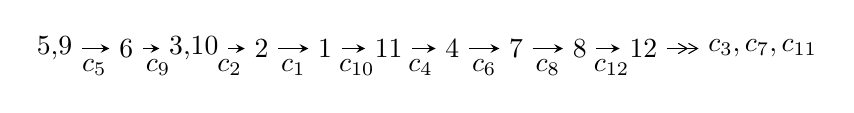
\begin{tikzpicture}[x=23pt, y=7pt]
	% node
	\node (A0) at (-1/8, 0) {5,9};
	\node (A1) at (1, 0) {6};
	\node (A2) at (33/16, 0) {3,10};
	\node (A3) at (25/8, 0) {2};
	\node (A4) at (33/8, 0) {1};
	\node (A5) at (41/8, 0) {11};
	\node (A6) at (49/8, 0) {4};
	\node (A7) at (57/8, 0) {7};
	\node (A8) at (65/8, 0) {8};
	\node (A9) at (73/8, 0) {12};
	\node (C1) at (1/2, -1) {$c_{5}$};
	\node (C2) at (3/2, -1) {$c_{9}$};
	\node (C3) at (21/8, -1) {$c_{2}$};
	\node (C4) at (29/8, -1) {$c_{1}$};
	\node (C5) at (37/8, -1) {$c_{10}$};
	\node (C6) at (45/8, -1) {$c_{4}$};
	\node (C7) at (53/8, -1) {$c_{6}$};
	\node (C8) at (61/8, -1) {$c_{8}$};
	\node (C9) at (69/8, -1) {$c_{12}$};
	\node (A10) at (11, 0) {$c_{3},c_{7},c_{11}$};

	% edge
	\draw[->,>=stealth]	
	(A0) edge (A1) (A1) edge (A2) (A2) edge (A3) (A3) edge (A4) (A4) edge (A5) (A5) edge (A6) (A6) edge (A7) (A7) edge (A8) (A8) edge (A9) ;
	\draw[->>,>={angle 60}]	
	(A9) edge (A10);
\end{tikzpicture} \\ 

\end{tabular} \\

\footnotetext{
The image of knot diagram is generated by the software ``\textbf{Draw programme}" developed by Andrew Bartholomew(\url{http://www.layer8.co.uk/maths/draw/index.htm\#Running-draw}), where we modified some parts for our purpose(\url{https://github.com/CATsTAILs/LinksPainter}).
}\phantom \\ \newline 
\centering \textbf{Ideals for irreducible components\footnotemark of $X_{\text{par}}$} 
 
\begin{align*}
I^u_{1}&=\langle 
-3.18936\times10^{246} u^{110}-2.13517\times10^{246} u^{109}+\cdots+5.64432\times10^{247} b-4.74907\times10^{248},\\
\phantom{I^u_{1}}&\phantom{= \langle  }4.40979\times10^{247} u^{110}+9.13393\times10^{247} u^{109}+\cdots+4.51546\times10^{248} a+1.43309\times10^{250},\\
\phantom{I^u_{1}}&\phantom{= \langle  }u^{111}+2 u^{110}+\cdots+160 u+64\rangle \\
I^u_{2}&=\langle 
b+1,\;- u^8+3 u^6+u^5-4 u^4-2 u^3+u^2+a+2 u+1,\;u^9+u^8-2 u^7-3 u^6+u^5+3 u^4+2 u^3- u-1\rangle \\
\\
I^v_{1}&=\langle 
a,\;-18 v^5+63 v^4-193 v^3+63 v^2+55 b+27 v-12,\;v^6-2 v^5+7 v^4+8 v^3+7 v^2+3 v+1\rangle \\
\end{align*}
\raggedright * 3 irreducible components of $\dim_{\mathbb{C}}=0$, with total 126 representations.\\
\footnotetext{All coefficients of polynomials are rational numbers. But the coefficients are sometimes approximated in decimal forms when there is not enough margin.}
\newpage
\renewcommand{\arraystretch}{1}
\centering \section*{I. $I^u_{1}= \langle -3.19\times10^{246} u^{110}-2.14\times10^{246} u^{109}+\cdots+5.64\times10^{247} b-4.75\times10^{248},\;4.41\times10^{247} u^{110}+9.13\times10^{247} u^{109}+\cdots+4.52\times10^{248} a+1.43\times10^{250},\;u^{111}+2 u^{110}+\cdots+160 u+64 \rangle$}
\flushleft \textbf{(i) Arc colorings}\\
\begin{tabular}{m{7pt} m{180pt} m{7pt} m{180pt} }
\flushright $a_{5}=$&$\begin{pmatrix}1\\0\end{pmatrix}$ \\
\flushright $a_{9}=$&$\begin{pmatrix}0\\u\end{pmatrix}$ \\
\flushright $a_{6}=$&$\begin{pmatrix}1\\u^2\end{pmatrix}$ \\
\flushright $a_{3}=$&$\begin{pmatrix}-0.0976599 u^{110}-0.202281 u^{109}+\cdots-0.854738 u-31.7375\\0.0565056 u^{110}+0.0378286 u^{109}+\cdots+22.9253 u+8.41389\end{pmatrix}$ \\
\flushright $a_{10}=$&$\begin{pmatrix}- u\\- u^3+u\end{pmatrix}$ \\
\flushright $a_{2}=$&$\begin{pmatrix}-0.0411543 u^{110}-0.164453 u^{109}+\cdots+22.0706 u-23.3236\\0.0565056 u^{110}+0.0378286 u^{109}+\cdots+22.9253 u+8.41389\end{pmatrix}$ \\
\flushright $a_{1}=$&$\begin{pmatrix}-0.120659 u^{110}-0.241271 u^{109}+\cdots-2.78514 u-16.8544\\0.0541953 u^{110}+0.118379 u^{109}+\cdots+2.44293 u-1.61000\end{pmatrix}$ \\
\flushright $a_{11}=$&$\begin{pmatrix}-0.143665 u^{110}-0.240646 u^{109}+\cdots-1.44973 u-16.5967\\0.0133269 u^{110}+0.0569514 u^{109}+\cdots-18.3902 u-8.25017\end{pmatrix}$ \\
\flushright $a_{4}=$&$\begin{pmatrix}0.0111189 u^{110}-0.0832837 u^{109}+\cdots+26.9485 u-9.66021\\0.0701195 u^{110}+0.127567 u^{109}+\cdots-6.36809 u+0.618737\end{pmatrix}$ \\
\flushright $a_{7}=$&$\begin{pmatrix}-0.0664640 u^{110}-0.122892 u^{109}+\cdots-0.342210 u-18.4644\\-0.0333772 u^{110}-0.0802479 u^{109}+\cdots+0.205002 u+0.967688\end{pmatrix}$ \\
\flushright $a_{8}=$&$\begin{pmatrix}u^3\\u^5- u^3+u\end{pmatrix}$ \\
\flushright $a_{12}=$&$\begin{pmatrix}-0.113592 u^{110}-0.203964 u^{109}+\cdots+0.640164 u-16.1869\\-0.0252501 u^{110}+0.0114473 u^{109}+\cdots-19.4565 u-11.8010\end{pmatrix}$\\&\end{tabular}
\flushleft \textbf{(ii) Obstruction class $= -1$}\\~\\
\flushleft \textbf{(iii) Cusp Shapes $= -0.161186 u^{110}-0.677696 u^{109}+\cdots+69.5252 u-36.2776$}\\~\\
\newpage\renewcommand{\arraystretch}{1}
\flushleft \textbf{(iv) u-Polynomials at the component}\newline \\
\begin{tabular}{m{50pt}|m{274pt}}
Crossings & \hspace{64pt}u-Polynomials at each crossing \\
\hline $$\begin{aligned}c_{1}\end{aligned}$$&$\begin{aligned}
&u^{111}+50 u^{110}+\cdots+45 u+1
\end{aligned}$\\
\hline $$\begin{aligned}c_{2},c_{4}\end{aligned}$$&$\begin{aligned}
&u^{111}-12 u^{110}+\cdots+u+1
\end{aligned}$\\
\hline $$\begin{aligned}c_{3},c_{6}\end{aligned}$$&$\begin{aligned}
&u^{111}-3 u^{110}+\cdots-2560 u+512
\end{aligned}$\\
\hline $$\begin{aligned}c_{5},c_{9}\end{aligned}$$&$\begin{aligned}
&u^{111}+2 u^{110}+\cdots+160 u+64
\end{aligned}$\\
\hline $$\begin{aligned}c_{7},c_{11}\end{aligned}$$&$\begin{aligned}
&u^{111}-5 u^{110}+\cdots+6 u+1
\end{aligned}$\\
\hline $$\begin{aligned}c_{8}\end{aligned}$$&$\begin{aligned}
&u^{111}+40 u^{110}+\cdots+107520 u+4096
\end{aligned}$\\
\hline $$\begin{aligned}c_{10},c_{12}\end{aligned}$$&$\begin{aligned}
&u^{111}-39 u^{110}+\cdots-34 u+1
\end{aligned}$\\
\hline
\end{tabular}\\~\\
\newpage\renewcommand{\arraystretch}{1}
\flushleft \textbf{(v) Riley Polynomials at the component}\newline \\
\begin{tabular}{m{50pt}|m{274pt}}
Crossings & \hspace{64pt}Riley Polynomials at each crossing \\
\hline $$\begin{aligned}c_{1}\end{aligned}$$&$\begin{aligned}
&y^{111}+34 y^{110}+\cdots-5587 y-1
\end{aligned}$\\
\hline $$\begin{aligned}c_{2},c_{4}\end{aligned}$$&$\begin{aligned}
&y^{111}-50 y^{110}+\cdots+45 y-1
\end{aligned}$\\
\hline $$\begin{aligned}c_{3},c_{6}\end{aligned}$$&$\begin{aligned}
&y^{111}+63 y^{110}+\cdots-3932160 y-262144
\end{aligned}$\\
\hline $$\begin{aligned}c_{5},c_{9}\end{aligned}$$&$\begin{aligned}
&y^{111}-40 y^{110}+\cdots+107520 y-4096
\end{aligned}$\\
\hline $$\begin{aligned}c_{7},c_{11}\end{aligned}$$&$\begin{aligned}
&y^{111}+39 y^{110}+\cdots-34 y-1
\end{aligned}$\\
\hline $$\begin{aligned}c_{8}\end{aligned}$$&$\begin{aligned}
&y^{111}+52 y^{110}+\cdots-334495744 y-16777216
\end{aligned}$\\
\hline $$\begin{aligned}c_{10},c_{12}\end{aligned}$$&$\begin{aligned}
&y^{111}+71 y^{110}+\cdots+250 y-1
\end{aligned}$\\
\hline
\end{tabular}\\~\\
\newpage\flushleft \textbf{(vi) Complex Volumes and Cusp Shapes}
$$\begin{array}{c|c|c}  
\text{Solutions to }I^u_{1}& \I (\text{vol} + \sqrt{-1}CS) & \text{Cusp shape}\\
 \hline 
\begin{aligned}
u &= \phantom{-}0.961261 + 0.305856 I \\
a &= \phantom{-}0.615473 - 0.767844 I \\
b &= \phantom{-}0.761803 - 0.469769 I\end{aligned}
 & \phantom{-}1.51893 - 1.34502 I & \phantom{-0.000000 } 0 \\ \hline\begin{aligned}
u &= \phantom{-}0.961261 - 0.305856 I \\
a &= \phantom{-}0.615473 + 0.767844 I \\
b &= \phantom{-}0.761803 + 0.469769 I\end{aligned}
 & \phantom{-}1.51893 + 1.34502 I & \phantom{-0.000000 } 0 \\ \hline\begin{aligned}
u &= -0.857490 + 0.495314 I \\
a &= -0.52751 - 2.40166 I \\
b &= -0.930489 + 0.464651 I\end{aligned}
 & -1.85472 + 3.13671 I & \phantom{-0.000000 } 0 \\ \hline\begin{aligned}
u &= -0.857490 - 0.495314 I \\
a &= -0.52751 + 2.40166 I \\
b &= -0.930489 - 0.464651 I\end{aligned}
 & -1.85472 - 3.13671 I & \phantom{-0.000000 } 0 \\ \hline\begin{aligned}
u &= \phantom{-}0.972722 + 0.028500 I \\
a &= \phantom{-}1.72566 + 0.16118 I \\
b &= \phantom{-}0.926889 + 0.540738 I\end{aligned}
 & \phantom{-}0.91466 - 5.55388 I & \phantom{-0.000000 } 0 \\ \hline\begin{aligned}
u &= \phantom{-}0.972722 - 0.028500 I \\
a &= \phantom{-}1.72566 - 0.16118 I \\
b &= \phantom{-}0.926889 - 0.540738 I\end{aligned}
 & \phantom{-}0.91466 + 5.55388 I & \phantom{-0.000000 } 0 \\ \hline\begin{aligned}
u &= \phantom{-}0.580825 + 0.879729 I \\
a &= \phantom{-}1.19720 - 1.21005 I \\
b &= -0.916016 + 0.511238 I\end{aligned}
 & -0.64800 + 5.40513 I & \phantom{-0.000000 } 0 \\ \hline\begin{aligned}
u &= \phantom{-}0.580825 - 0.879729 I \\
a &= \phantom{-}1.19720 + 1.21005 I \\
b &= -0.916016 - 0.511238 I\end{aligned}
 & -0.64800 - 5.40513 I & \phantom{-0.000000 } 0 \\ \hline\begin{aligned}
u &= -0.765501 + 0.553121 I \\
a &= -0.500470 - 1.110230 I \\
b &= \phantom{-}1.029320 + 0.785263 I\end{aligned}
 & \phantom{-}3.64520 + 0.60285 I & \phantom{-0.000000 } 0 \\ \hline\begin{aligned}
u &= -0.765501 - 0.553121 I \\
a &= -0.500470 + 1.110230 I \\
b &= \phantom{-}1.029320 - 0.785263 I\end{aligned}
 & \phantom{-}3.64520 - 0.60285 I & \phantom{-0.000000 } 0\\
 \hline 
 \end{array}$$\newpage$$\begin{array}{c|c|c}  
\text{Solutions to }I^u_{1}& \I (\text{vol} + \sqrt{-1}CS) & \text{Cusp shape}\\
 \hline 
\begin{aligned}
u &= \phantom{-}0.716525 + 0.613563 I \\
a &= -0.153728 - 1.308980 I \\
b &= \phantom{-}0.689023 + 0.854328 I\end{aligned}
 & \phantom{-}3.48851 - 1.75426 I & \phantom{-0.000000 } 0 \\ \hline\begin{aligned}
u &= \phantom{-}0.716525 - 0.613563 I \\
a &= -0.153728 + 1.308980 I \\
b &= \phantom{-}0.689023 - 0.854328 I\end{aligned}
 & \phantom{-}3.48851 + 1.75426 I & \phantom{-0.000000 } 0 \\ \hline\begin{aligned}
u &= \phantom{-}0.788393 + 0.725909 I \\
a &= \phantom{-}1.10459 - 1.09562 I \\
b &= -0.781000 + 0.575014 I\end{aligned}
 & \phantom{-}3.15897 - 0.41518 I & \phantom{-0.000000 } 0 \\ \hline\begin{aligned}
u &= \phantom{-}0.788393 - 0.725909 I \\
a &= \phantom{-}1.10459 + 1.09562 I \\
b &= -0.781000 - 0.575014 I\end{aligned}
 & \phantom{-}3.15897 + 0.41518 I & \phantom{-0.000000 } 0 \\ \hline\begin{aligned}
u &= -0.849847 + 0.655093 I \\
a &= -0.165620 + 1.385900 I \\
b &= \phantom{-}0.674325 - 0.922324 I\end{aligned}
 & \phantom{-}4.71931 + 6.83549 I & \phantom{-0.000000 } 0 \\ \hline\begin{aligned}
u &= -0.849847 - 0.655093 I \\
a &= -0.165620 - 1.385900 I \\
b &= \phantom{-}0.674325 + 0.922324 I\end{aligned}
 & \phantom{-}4.71931 - 6.83549 I & \phantom{-0.000000 } 0 \\ \hline\begin{aligned}
u &= -0.472703 + 0.795398 I \\
a &= \phantom{-}1.28208 + 1.21302 I \\
b &= -0.908601 - 0.434969 I\end{aligned}
 & -1.65724 - 0.25812 I & \phantom{-0.000000 } 0 \\ \hline\begin{aligned}
u &= -0.472703 - 0.795398 I \\
a &= \phantom{-}1.28208 - 1.21302 I \\
b &= -0.908601 + 0.434969 I\end{aligned}
 & -1.65724 + 0.25812 I & \phantom{-0.000000 } 0 \\ \hline\begin{aligned}
u &= -0.847842 + 0.674035 I \\
a &= -0.296981 - 0.910876 I \\
b &= -1.294380 - 0.050287 I\end{aligned}
 & \phantom{-}1.45768 + 2.60301 I & \phantom{-0.000000 } 0 \\ \hline\begin{aligned}
u &= -0.847842 - 0.674035 I \\
a &= -0.296981 + 0.910876 I \\
b &= -1.294380 + 0.050287 I\end{aligned}
 & \phantom{-}1.45768 - 2.60301 I & \phantom{-0.000000 } 0\\
 \hline 
 \end{array}$$\newpage$$\begin{array}{c|c|c}  
\text{Solutions to }I^u_{1}& \I (\text{vol} + \sqrt{-1}CS) & \text{Cusp shape}\\
 \hline 
\begin{aligned}
u &= -0.500463 + 0.766009 I \\
a &= \phantom{-}0.15270 - 1.69929 I \\
b &= -1.219930 + 0.077295 I\end{aligned}
 & -1.75055 - 3.19219 I & \phantom{-0.000000 } 0 \\ \hline\begin{aligned}
u &= -0.500463 - 0.766009 I \\
a &= \phantom{-}0.15270 + 1.69929 I \\
b &= -1.219930 - 0.077295 I\end{aligned}
 & -1.75055 + 3.19219 I & \phantom{-0.000000 } 0 \\ \hline\begin{aligned}
u &= -1.077640 + 0.129946 I \\
a &= \phantom{-}0.361937 - 0.584101 I \\
b &= -0.084940 + 0.655027 I\end{aligned}
 & -4.12746 - 0.17488 I & \phantom{-0.000000 } 0 \\ \hline\begin{aligned}
u &= -1.077640 - 0.129946 I \\
a &= \phantom{-}0.361937 + 0.584101 I \\
b &= -0.084940 - 0.655027 I\end{aligned}
 & -4.12746 + 0.17488 I & \phantom{-0.000000 } 0 \\ \hline\begin{aligned}
u &= -0.074865 + 1.083460 I \\
a &= -0.251254 + 0.791988 I \\
b &= \phantom{-}0.912226 - 0.474868 I\end{aligned}
 & -1.46708 + 4.63529 I & \phantom{-0.000000 } 0 \\ \hline\begin{aligned}
u &= -0.074865 - 1.083460 I \\
a &= -0.251254 - 0.791988 I \\
b &= \phantom{-}0.912226 + 0.474868 I\end{aligned}
 & -1.46708 - 4.63529 I & \phantom{-0.000000 } 0 \\ \hline\begin{aligned}
u &= -0.690756 + 0.843068 I \\
a &= -0.535950 - 1.011050 I \\
b &= \phantom{-}1.080660 + 0.712649 I\end{aligned}
 & \phantom{-}6.97174 - 5.31220 I & \phantom{-0.000000 } 0 \\ \hline\begin{aligned}
u &= -0.690756 - 0.843068 I \\
a &= -0.535950 + 1.011050 I \\
b &= \phantom{-}1.080660 - 0.712649 I\end{aligned}
 & \phantom{-}6.97174 + 5.31220 I & \phantom{-0.000000 } 0 \\ \hline\begin{aligned}
u &= -0.956831 + 0.525019 I \\
a &= \phantom{-}0.954350 + 0.985429 I \\
b &= -0.621966 - 0.625924 I\end{aligned}
 & -2.27963 + 0.82457 I & \phantom{-0.000000 } 0 \\ \hline\begin{aligned}
u &= -0.956831 - 0.525019 I \\
a &= \phantom{-}0.954350 - 0.985429 I \\
b &= -0.621966 + 0.625924 I\end{aligned}
 & -2.27963 - 0.82457 I & \phantom{-0.000000 } 0\\
 \hline 
 \end{array}$$\newpage$$\begin{array}{c|c|c}  
\text{Solutions to }I^u_{1}& \I (\text{vol} + \sqrt{-1}CS) & \text{Cusp shape}\\
 \hline 
\begin{aligned}
u &= \phantom{-}0.192505 + 1.075250 I \\
a &= -0.177114 - 0.778854 I \\
b &= \phantom{-}0.860535 + 0.445165 I\end{aligned}
 & -1.23200 + 0.90790 I & \phantom{-0.000000 } 0 \\ \hline\begin{aligned}
u &= \phantom{-}0.192505 - 1.075250 I \\
a &= -0.177114 + 0.778854 I \\
b &= \phantom{-}0.860535 - 0.445165 I\end{aligned}
 & -1.23200 - 0.90790 I & \phantom{-0.000000 } 0 \\ \hline\begin{aligned}
u &= -0.859755 + 0.675252 I \\
a &= -1.135270 - 0.160639 I \\
b &= \phantom{-}0.532972 + 0.838336 I\end{aligned}
 & \phantom{-}4.68879 - 1.68552 I & \phantom{-0.000000 } 0 \\ \hline\begin{aligned}
u &= -0.859755 - 0.675252 I \\
a &= -1.135270 + 0.160639 I \\
b &= \phantom{-}0.532972 - 0.838336 I\end{aligned}
 & \phantom{-}4.68879 + 1.68552 I & \phantom{-0.000000 } 0 \\ \hline\begin{aligned}
u &= -0.945558 + 0.570571 I \\
a &= \phantom{-}1.26787 + 2.01034 I \\
b &= \phantom{-}1.077520 - 0.661944 I\end{aligned}
 & \phantom{-}3.04138 + 3.90587 I & \phantom{-0.000000 } 0 \\ \hline\begin{aligned}
u &= -0.945558 - 0.570571 I \\
a &= \phantom{-}1.26787 - 2.01034 I \\
b &= \phantom{-}1.077520 + 0.661944 I\end{aligned}
 & \phantom{-}3.04138 - 3.90587 I & \phantom{-0.000000 } 0 \\ \hline\begin{aligned}
u &= \phantom{-}0.664358 + 0.599954 I \\
a &= -0.08780 + 2.94975 I \\
b &= -0.802872 - 0.455801 I\end{aligned}
 & -0.20502 + 1.39970 I & \phantom{-0.000000 } 0 \\ \hline\begin{aligned}
u &= \phantom{-}0.664358 - 0.599954 I \\
a &= -0.08780 - 2.94975 I \\
b &= -0.802872 + 0.455801 I\end{aligned}
 & -0.20502 - 1.39970 I & \phantom{-0.000000 } 0 \\ \hline\begin{aligned}
u &= \phantom{-}0.641635 + 0.909705 I \\
a &= \phantom{-}0.072845 - 1.364280 I \\
b &= \phantom{-}0.486017 + 0.821449 I\end{aligned}
 & \phantom{-}2.97384 + 0.23222 I & \phantom{-0.000000 } 0 \\ \hline\begin{aligned}
u &= \phantom{-}0.641635 - 0.909705 I \\
a &= \phantom{-}0.072845 + 1.364280 I \\
b &= \phantom{-}0.486017 - 0.821449 I\end{aligned}
 & \phantom{-}2.97384 - 0.23222 I & \phantom{-0.000000 } 0\\
 \hline 
 \end{array}$$\newpage$$\begin{array}{c|c|c}  
\text{Solutions to }I^u_{1}& \I (\text{vol} + \sqrt{-1}CS) & \text{Cusp shape}\\
 \hline 
\begin{aligned}
u &= -1.112920 + 0.132238 I \\
a &= \phantom{-}1.000340 + 0.261885 I \\
b &= \phantom{-}0.897392 + 0.447328 I\end{aligned}
 & -2.09929 - 1.79300 I & \phantom{-0.000000 } 0 \\ \hline\begin{aligned}
u &= -1.112920 - 0.132238 I \\
a &= \phantom{-}1.000340 - 0.261885 I \\
b &= \phantom{-}0.897392 - 0.447328 I\end{aligned}
 & -2.09929 + 1.79300 I & \phantom{-0.000000 } 0 \\ \hline\begin{aligned}
u &= \phantom{-}1.100350 + 0.229120 I \\
a &= \phantom{-}0.212933 + 0.553604 I \\
b &= \phantom{-}0.005517 - 0.693265 I\end{aligned}
 & -3.81029 - 5.38817 I & \phantom{-0.000000 } 0 \\ \hline\begin{aligned}
u &= \phantom{-}1.100350 - 0.229120 I \\
a &= \phantom{-}0.212933 - 0.553604 I \\
b &= \phantom{-}0.005517 + 0.693265 I\end{aligned}
 & -3.81029 + 5.38817 I & \phantom{-0.000000 } 0 \\ \hline\begin{aligned}
u &= -0.773381 + 0.830007 I \\
a &= -0.048570 + 1.407420 I \\
b &= \phantom{-}0.568998 - 0.900673 I\end{aligned}
 & \phantom{-}8.52723 + 0.62332 I & \phantom{-0.000000 } 0 \\ \hline\begin{aligned}
u &= -0.773381 - 0.830007 I \\
a &= -0.048570 - 1.407420 I \\
b &= \phantom{-}0.568998 + 0.900673 I\end{aligned}
 & \phantom{-}8.52723 - 0.62332 I & \phantom{-0.000000 } 0 \\ \hline\begin{aligned}
u &= \phantom{-}0.938382 + 0.649116 I \\
a &= -0.861937 + 0.269194 I \\
b &= \phantom{-}0.464394 - 0.835909 I\end{aligned}
 & \phantom{-}2.81501 - 3.26360 I & \phantom{-0.000000 } 0 \\ \hline\begin{aligned}
u &= \phantom{-}0.938382 - 0.649116 I \\
a &= -0.861937 - 0.269194 I \\
b &= \phantom{-}0.464394 + 0.835909 I\end{aligned}
 & \phantom{-}2.81501 + 3.26360 I & \phantom{-0.000000 } 0 \\ \hline\begin{aligned}
u &= \phantom{-}0.913223 + 0.693999 I \\
a &= -0.06671 + 2.28822 I \\
b &= -0.901738 - 0.574717 I\end{aligned}
 & \phantom{-}2.77609 - 5.00482 I & \phantom{-0.000000 } 0 \\ \hline\begin{aligned}
u &= \phantom{-}0.913223 - 0.693999 I \\
a &= -0.06671 - 2.28822 I \\
b &= -0.901738 + 0.574717 I\end{aligned}
 & \phantom{-}2.77609 + 5.00482 I & \phantom{-0.000000 } 0\\
 \hline 
 \end{array}$$\newpage$$\begin{array}{c|c|c}  
\text{Solutions to }I^u_{1}& \I (\text{vol} + \sqrt{-1}CS) & \text{Cusp shape}\\
 \hline 
\begin{aligned}
u &= \phantom{-}0.778898 + 0.343012 I \\
a &= -1.41652 + 0.71580 I \\
b &= -1.176390 + 0.127517 I\end{aligned}
 & -2.73805 - 1.01723 I & -10.94783 + 6.27439 I \\ \hline\begin{aligned}
u &= \phantom{-}0.778898 - 0.343012 I \\
a &= -1.41652 - 0.71580 I \\
b &= -1.176390 - 0.127517 I\end{aligned}
 & -2.73805 + 1.01723 I & -10.94783 - 6.27439 I \\ \hline\begin{aligned}
u &= \phantom{-}1.153030 + 0.000762 I \\
a &= -0.760894 + 0.885736 I \\
b &= -1.195590 - 0.353101 I\end{aligned}
 & -7.47764 + 1.50835 I & \phantom{-0.000000 } 0 \\ \hline\begin{aligned}
u &= \phantom{-}1.153030 - 0.000762 I \\
a &= -0.760894 - 0.885736 I \\
b &= -1.195590 + 0.353101 I\end{aligned}
 & -7.47764 - 1.50835 I & \phantom{-0.000000 } 0 \\ \hline\begin{aligned}
u &= -1.157080 + 0.095057 I \\
a &= -0.720181 - 1.109600 I \\
b &= -1.170490 + 0.388339 I\end{aligned}
 & -7.39457 + 4.16403 I & \phantom{-0.000000 } 0 \\ \hline\begin{aligned}
u &= -1.157080 - 0.095057 I \\
a &= -0.720181 + 1.109600 I \\
b &= -1.170490 - 0.388339 I\end{aligned}
 & -7.39457 - 4.16403 I & \phantom{-0.000000 } 0 \\ \hline\begin{aligned}
u &= \phantom{-}0.993165 + 0.613622 I \\
a &= \phantom{-}0.95705 - 1.05542 I \\
b &= -0.669117 + 0.666637 I\end{aligned}
 & -1.23032 - 6.24800 I & \phantom{-0.000000 } 0 \\ \hline\begin{aligned}
u &= \phantom{-}0.993165 - 0.613622 I \\
a &= \phantom{-}0.95705 + 1.05542 I \\
b &= -0.669117 - 0.666637 I\end{aligned}
 & -1.23032 + 6.24800 I & \phantom{-0.000000 } 0 \\ \hline\begin{aligned}
u &= \phantom{-}0.571056 + 1.026180 I \\
a &= -0.532528 + 0.924418 I \\
b &= \phantom{-}1.096700 - 0.642791 I\end{aligned}
 & \phantom{-}1.13791 + 5.71377 I & \phantom{-0.000000 } 0 \\ \hline\begin{aligned}
u &= \phantom{-}0.571056 - 1.026180 I \\
a &= -0.532528 - 0.924418 I \\
b &= \phantom{-}1.096700 + 0.642791 I\end{aligned}
 & \phantom{-}1.13791 - 5.71377 I & \phantom{-0.000000 } 0\\
 \hline 
 \end{array}$$\newpage$$\begin{array}{c|c|c}  
\text{Solutions to }I^u_{1}& \I (\text{vol} + \sqrt{-1}CS) & \text{Cusp shape}\\
 \hline 
\begin{aligned}
u &= -0.688824 + 0.955138 I \\
a &= \phantom{-}0.07067 + 1.42628 I \\
b &= \phantom{-}0.464226 - 0.871917 I\end{aligned}
 & \phantom{-}4.21683 - 5.60824 I & \phantom{-0.000000 } 0 \\ \hline\begin{aligned}
u &= -0.688824 - 0.955138 I \\
a &= \phantom{-}0.07067 - 1.42628 I \\
b &= \phantom{-}0.464226 + 0.871917 I\end{aligned}
 & \phantom{-}4.21683 + 5.60824 I & \phantom{-0.000000 } 0 \\ \hline\begin{aligned}
u &= \phantom{-}0.686909 + 0.436600 I \\
a &= \phantom{-}0.496822 - 0.215720 I \\
b &= \phantom{-}0.236693 - 0.173944 I\end{aligned}
 & \phantom{-}1.43635 - 1.82704 I & -0.84954 + 4.84948 I \\ \hline\begin{aligned}
u &= \phantom{-}0.686909 - 0.436600 I \\
a &= \phantom{-}0.496822 + 0.215720 I \\
b &= \phantom{-}0.236693 + 0.173944 I\end{aligned}
 & \phantom{-}1.43635 + 1.82704 I & -0.84954 - 4.84948 I \\ \hline\begin{aligned}
u &= \phantom{-}1.044800 + 0.576162 I \\
a &= -0.348684 + 0.417955 I \\
b &= -1.324720 + 0.135388 I\end{aligned}
 & -4.45792 - 2.96094 I & \phantom{-0.000000 } 0 \\ \hline\begin{aligned}
u &= \phantom{-}1.044800 - 0.576162 I \\
a &= -0.348684 - 0.417955 I \\
b &= -1.324720 - 0.135388 I\end{aligned}
 & -4.45792 + 2.96094 I & \phantom{-0.000000 } 0 \\ \hline\begin{aligned}
u &= \phantom{-}1.052210 + 0.597069 I \\
a &= \phantom{-}0.98408 - 1.77129 I \\
b &= \phantom{-}1.109350 + 0.642860 I\end{aligned}
 & \phantom{-}0.87796 - 8.78070 I & \phantom{-0.000000 } 0 \\ \hline\begin{aligned}
u &= \phantom{-}1.052210 - 0.597069 I \\
a &= \phantom{-}0.98408 + 1.77129 I \\
b &= \phantom{-}1.109350 - 0.642860 I\end{aligned}
 & \phantom{-}0.87796 + 8.78070 I & \phantom{-0.000000 } 0 \\ \hline\begin{aligned}
u &= \phantom{-}0.362203 + 0.687116 I \\
a &= -0.405923 + 1.008540 I \\
b &= \phantom{-}0.977149 - 0.680548 I\end{aligned}
 & \phantom{-}2.67743 + 3.92833 I & -5.69908 - 2.39283 I \\ \hline\begin{aligned}
u &= \phantom{-}0.362203 - 0.687116 I \\
a &= -0.405923 - 1.008540 I \\
b &= \phantom{-}0.977149 + 0.680548 I\end{aligned}
 & \phantom{-}2.67743 - 3.92833 I & -5.69908 + 2.39283 I\\
 \hline 
 \end{array}$$\newpage$$\begin{array}{c|c|c}  
\text{Solutions to }I^u_{1}& \I (\text{vol} + \sqrt{-1}CS) & \text{Cusp shape}\\
 \hline 
\begin{aligned}
u &= -0.969355 + 0.753597 I \\
a &= -0.991867 - 0.557856 I \\
b &= \phantom{-}0.475097 + 0.920853 I\end{aligned}
 & \phantom{-}7.90957 + 5.29556 I & \phantom{-0.000000 } 0 \\ \hline\begin{aligned}
u &= -0.969355 - 0.753597 I \\
a &= -0.991867 + 0.557856 I \\
b &= \phantom{-}0.475097 - 0.920853 I\end{aligned}
 & \phantom{-}7.90957 - 5.29556 I & \phantom{-0.000000 } 0 \\ \hline\begin{aligned}
u &= -0.645356 + 1.047180 I \\
a &= -0.563660 - 0.932862 I \\
b &= \phantom{-}1.119580 + 0.656047 I\end{aligned}
 & \phantom{-}2.23809 - 11.26390 I & \phantom{-0.000000 } 0 \\ \hline\begin{aligned}
u &= -0.645356 - 1.047180 I \\
a &= -0.563660 + 0.932862 I \\
b &= \phantom{-}1.119580 - 0.656047 I\end{aligned}
 & \phantom{-}2.23809 + 11.26390 I & \phantom{-0.000000 } 0 \\ \hline\begin{aligned}
u &= -1.059270 + 0.647902 I \\
a &= -0.207983 - 0.464083 I \\
b &= -1.349170 - 0.118043 I\end{aligned}
 & -3.35615 + 8.53993 I & \phantom{-0.000000 } 0 \\ \hline\begin{aligned}
u &= -1.059270 - 0.647902 I \\
a &= -0.207983 + 0.464083 I \\
b &= -1.349170 + 0.118043 I\end{aligned}
 & -3.35615 - 8.53993 I & \phantom{-0.000000 } 0 \\ \hline\begin{aligned}
u &= -1.066380 + 0.641788 I \\
a &= -0.12862 - 2.02884 I \\
b &= -0.986679 + 0.588452 I\end{aligned}
 & -3.37073 + 5.61350 I & \phantom{-0.000000 } 0 \\ \hline\begin{aligned}
u &= -1.066380 - 0.641788 I \\
a &= -0.12862 + 2.02884 I \\
b &= -0.986679 - 0.588452 I\end{aligned}
 & -3.37073 - 5.61350 I & \phantom{-0.000000 } 0 \\ \hline\begin{aligned}
u &= \phantom{-}0.267839 + 0.699470 I \\
a &= \phantom{-}0.68721 + 2.21087 I \\
b &= -1.129410 - 0.124638 I\end{aligned}
 & -2.49151 - 1.68594 I & -7.47036 - 1.42690 I \\ \hline\begin{aligned}
u &= \phantom{-}0.267839 - 0.699470 I \\
a &= \phantom{-}0.68721 - 2.21087 I \\
b &= -1.129410 + 0.124638 I\end{aligned}
 & -2.49151 + 1.68594 I & -7.47036 + 1.42690 I\\
 \hline 
 \end{array}$$\newpage$$\begin{array}{c|c|c}  
\text{Solutions to }I^u_{1}& \I (\text{vol} + \sqrt{-1}CS) & \text{Cusp shape}\\
 \hline 
\begin{aligned}
u &= -1.030160 + 0.720587 I \\
a &= \phantom{-}0.71254 + 2.00743 I \\
b &= \phantom{-}1.132590 - 0.678871 I\end{aligned}
 & \phantom{-}5.90690 + 11.16420 I & \phantom{-0.000000 } 0 \\ \hline\begin{aligned}
u &= -1.030160 - 0.720587 I \\
a &= \phantom{-}0.71254 - 2.00743 I \\
b &= \phantom{-}1.132590 + 0.678871 I\end{aligned}
 & \phantom{-}5.90690 - 11.16420 I & \phantom{-0.000000 } 0 \\ \hline\begin{aligned}
u &= \phantom{-}1.077120 + 0.699464 I \\
a &= -0.04264 + 2.03440 I \\
b &= -0.977779 - 0.617324 I\end{aligned}
 & -2.17058 - 11.24930 I & \phantom{-0.000000 } 0 \\ \hline\begin{aligned}
u &= \phantom{-}1.077120 - 0.699464 I \\
a &= -0.04264 - 2.03440 I \\
b &= -0.977779 + 0.617324 I\end{aligned}
 & -2.17058 + 11.24930 I & \phantom{-0.000000 } 0 \\ \hline\begin{aligned}
u &= \phantom{-}1.066800 + 0.727963 I \\
a &= -0.777069 + 0.660416 I \\
b &= \phantom{-}0.404198 - 0.940500 I\end{aligned}
 & \phantom{-}1.63590 - 6.26824 I & \phantom{-0.000000 } 0 \\ \hline\begin{aligned}
u &= \phantom{-}1.066800 - 0.727963 I \\
a &= -0.777069 - 0.660416 I \\
b &= \phantom{-}0.404198 + 0.940500 I\end{aligned}
 & \phantom{-}1.63590 + 6.26824 I & \phantom{-0.000000 } 0 \\ \hline\begin{aligned}
u &= \phantom{-}0.611834 + 0.346825 I \\
a &= -0.424809 + 1.132140 I \\
b &= \phantom{-}0.961999 - 0.784969 I\end{aligned}
 & \phantom{-}2.73478 + 4.20900 I & -10.00721 + 0.57642 I \\ \hline\begin{aligned}
u &= \phantom{-}0.611834 - 0.346825 I \\
a &= -0.424809 - 1.132140 I \\
b &= \phantom{-}0.961999 + 0.784969 I\end{aligned}
 & \phantom{-}2.73478 - 4.20900 I & -10.00721 - 0.57642 I \\ \hline\begin{aligned}
u &= \phantom{-}0.424597 + 0.530789 I \\
a &= -0.188404 - 1.154690 I \\
b &= \phantom{-}0.764069 + 0.739282 I\end{aligned}
 & \phantom{-}3.38545 - 1.57723 I & -2.69554 + 5.44980 I \\ \hline\begin{aligned}
u &= \phantom{-}0.424597 - 0.530789 I \\
a &= -0.188404 + 1.154690 I \\
b &= \phantom{-}0.764069 - 0.739282 I\end{aligned}
 & \phantom{-}3.38545 + 1.57723 I & -2.69554 - 5.44980 I\\
 \hline 
 \end{array}$$\newpage$$\begin{array}{c|c|c}  
\text{Solutions to }I^u_{1}& \I (\text{vol} + \sqrt{-1}CS) & \text{Cusp shape}\\
 \hline 
\begin{aligned}
u &= -1.075540 + 0.768246 I \\
a &= -0.821553 - 0.734422 I \\
b &= \phantom{-}0.415395 + 0.967932 I\end{aligned}
 & \phantom{-}2.97459 + 11.93470 I & \phantom{-0.000000 } 0 \\ \hline\begin{aligned}
u &= -1.075540 - 0.768246 I \\
a &= -0.821553 + 0.734422 I \\
b &= \phantom{-}0.415395 - 0.967932 I\end{aligned}
 & \phantom{-}2.97459 - 11.93470 I & \phantom{-0.000000 } 0 \\ \hline\begin{aligned}
u &= -1.265160 + 0.437949 I \\
a &= \phantom{-}0.471571 + 0.242610 I \\
b &= \phantom{-}0.848355 + 0.276852 I\end{aligned}
 & -5.56887 + 0.59401 I & \phantom{-0.000000 } 0 \\ \hline\begin{aligned}
u &= -1.265160 - 0.437949 I \\
a &= \phantom{-}0.471571 - 0.242610 I \\
b &= \phantom{-}0.848355 - 0.276852 I\end{aligned}
 & -5.56887 - 0.59401 I & \phantom{-0.000000 } 0 \\ \hline\begin{aligned}
u &= -1.333270 + 0.173414 I \\
a &= \phantom{-}0.837831 + 0.522328 I \\
b &= \phantom{-}1.063820 - 0.455497 I\end{aligned}
 & -6.98403 + 3.40230 I & \phantom{-0.000000 } 0 \\ \hline\begin{aligned}
u &= -1.333270 - 0.173414 I \\
a &= \phantom{-}0.837831 - 0.522328 I \\
b &= \phantom{-}1.063820 + 0.455497 I\end{aligned}
 & -6.98403 - 3.40230 I & \phantom{-0.000000 } 0 \\ \hline\begin{aligned}
u &= \phantom{-}1.325960 + 0.257152 I \\
a &= \phantom{-}0.835359 - 0.688269 I \\
b &= \phantom{-}1.087480 + 0.480695 I\end{aligned}
 & -6.62780 - 9.38031 I & \phantom{-0.000000 } 0 \\ \hline\begin{aligned}
u &= \phantom{-}1.325960 - 0.257152 I \\
a &= \phantom{-}0.835359 + 0.688269 I \\
b &= \phantom{-}1.087480 - 0.480695 I\end{aligned}
 & -6.62780 + 9.38031 I & \phantom{-0.000000 } 0 \\ \hline\begin{aligned}
u &= \phantom{-}1.246820 + 0.525991 I \\
a &= \phantom{-}0.407713 - 0.268068 I \\
b &= \phantom{-}0.821780 - 0.240489 I\end{aligned}
 & -4.75429 - 6.49311 I & \phantom{-0.000000 } 0 \\ \hline\begin{aligned}
u &= \phantom{-}1.246820 - 0.525991 I \\
a &= \phantom{-}0.407713 + 0.268068 I \\
b &= \phantom{-}0.821780 + 0.240489 I\end{aligned}
 & -4.75429 + 6.49311 I & \phantom{-0.000000 } 0\\
 \hline 
 \end{array}$$\newpage$$\begin{array}{c|c|c}  
\text{Solutions to }I^u_{1}& \I (\text{vol} + \sqrt{-1}CS) & \text{Cusp shape}\\
 \hline 
\begin{aligned}
u &= \phantom{-}1.142380 + 0.741212 I \\
a &= \phantom{-}0.54160 - 1.78118 I \\
b &= \phantom{-}1.166410 + 0.658674 I\end{aligned}
 & -0.68346 - 12.10710 I & \phantom{-0.000000 } 0 \\ \hline\begin{aligned}
u &= \phantom{-}1.142380 - 0.741212 I \\
a &= \phantom{-}0.54160 + 1.78118 I \\
b &= \phantom{-}1.166410 - 0.658674 I\end{aligned}
 & -0.68346 + 12.10710 I & \phantom{-0.000000 } 0 \\ \hline\begin{aligned}
u &= -1.135360 + 0.783517 I \\
a &= \phantom{-}0.46510 + 1.83815 I \\
b &= \phantom{-}1.174150 - 0.671550 I\end{aligned}
 & \phantom{-}0.6511 + 17.8984 I & \phantom{-0.000000 } 0 \\ \hline\begin{aligned}
u &= -1.135360 - 0.783517 I \\
a &= \phantom{-}0.46510 - 1.83815 I \\
b &= \phantom{-}1.174150 + 0.671550 I\end{aligned}
 & \phantom{-}0.6511 - 17.8984 I & \phantom{-0.000000 } 0 \\ \hline\begin{aligned}
u &= -0.597936\phantom{ +0.000000I} \\
a &= \phantom{-}0.991036\phantom{ +0.000000I} \\
b &= -0.266692\phantom{ +0.000000I}\end{aligned}
 & -0.855489\phantom{ +0.000000I} & -11.6530\phantom{ +0.000000I} \\ \hline\begin{aligned}
u &= \phantom{-}0.078117 + 0.575284 I \\
a &= \phantom{-}1.54993 - 0.43215 I \\
b &= -0.0983081 + 0.0963811 I\end{aligned}
 & -0.46663 + 2.30779 I & -1.91194 - 3.67862 I \\ \hline\begin{aligned}
u &= \phantom{-}0.078117 - 0.575284 I \\
a &= \phantom{-}1.54993 + 0.43215 I \\
b &= -0.0983081 - 0.0963811 I\end{aligned}
 & -0.46663 - 2.30779 I & -1.91194 + 3.67862 I \\ \hline\begin{aligned}
u &= -0.379391 + 0.286023 I \\
a &= \phantom{-}1.65758 + 0.59289 I \\
b &= -0.700392 - 0.183066 I\end{aligned}
 & -0.947135 - 0.090988 I & -9.16846 - 0.70332 I \\ \hline\begin{aligned}
u &= -0.379391 - 0.286023 I \\
a &= \phantom{-}1.65758 - 0.59289 I \\
b &= -0.700392 + 0.183066 I\end{aligned}
 & -0.947135 + 0.090988 I & -9.16846 + 0.70332 I \\ \hline\begin{aligned}
u &= -0.464260 + 0.090617 I \\
a &= -5.72829 - 3.35406 I \\
b &= -0.913336 + 0.139185 I\end{aligned}
 & -1.26665 + 2.32355 I & -25.1036 - 5.2591 I\\
 \hline 
 \end{array}$$\newpage$$\begin{array}{c|c|c}  
\text{Solutions to }I^u_{1}& \I (\text{vol} + \sqrt{-1}CS) & \text{Cusp shape}\\
 \hline 
\begin{aligned}
u &= -0.464260 - 0.090617 I \\
a &= -5.72829 + 3.35406 I \\
b &= -0.913336 - 0.139185 I\end{aligned}
 & -1.26665 - 2.32355 I & -25.1036 + 5.2591 I\\
 \hline 
 \end{array}$$\newpage\newpage\renewcommand{\arraystretch}{1}
\centering \section*{II. $I^u_{2}= \langle b+1,\;- u^8+3 u^6+u^5-4 u^4-2 u^3+u^2+a+2 u+1,\;u^9+u^8-2 u^7-3 u^6+u^5+3 u^4+2 u^3- u-1 \rangle$}
\flushleft \textbf{(i) Arc colorings}\\
\begin{tabular}{m{7pt} m{180pt} m{7pt} m{180pt} }
\flushright $a_{5}=$&$\begin{pmatrix}1\\0\end{pmatrix}$ \\
\flushright $a_{9}=$&$\begin{pmatrix}0\\u\end{pmatrix}$ \\
\flushright $a_{6}=$&$\begin{pmatrix}1\\u^2\end{pmatrix}$ \\
\flushright $a_{3}=$&$\begin{pmatrix}u^8-3 u^6- u^5+4 u^4+2 u^3- u^2-2 u-1\\-1\end{pmatrix}$ \\
\flushright $a_{10}=$&$\begin{pmatrix}- u\\- u^3+u\end{pmatrix}$ \\
\flushright $a_{2}=$&$\begin{pmatrix}u^8-3 u^6- u^5+4 u^4+2 u^3- u^2-2 u-2\\-1\end{pmatrix}$ \\
\flushright $a_{1}=$&$\begin{pmatrix}-1\\0\end{pmatrix}$ \\
\flushright $a_{11}=$&$\begin{pmatrix}- u^3\\- u^3+u\end{pmatrix}$ \\
\flushright $a_{4}=$&$\begin{pmatrix}u^8-3 u^6- u^5+4 u^4+2 u^3- u^2-2 u-1\\-1\end{pmatrix}$ \\
\flushright $a_{7}=$&$\begin{pmatrix}1\\u^2\end{pmatrix}$ \\
\flushright $a_{8}=$&$\begin{pmatrix}u^3\\u^5- u^3+u\end{pmatrix}$ \\
\flushright $a_{12}=$&$\begin{pmatrix}- u^6+u^4-1\\- u^6+2 u^4- u^2\end{pmatrix}$\\&\end{tabular}
\flushleft \textbf{(ii) Obstruction class $= 1$}\\~\\
\flushleft \textbf{(iii) Cusp Shapes $= u^8-2 u^7-2 u^6+3 u^5+6 u^4-3 u^3-3 u^2-4 u-10$}\\~\\
\newpage\renewcommand{\arraystretch}{1}
\flushleft \textbf{(iv) u-Polynomials at the component}\newline \\
\begin{tabular}{m{50pt}|m{274pt}}
Crossings & \hspace{64pt}u-Polynomials at each crossing \\
\hline $$\begin{aligned}c_{1},c_{2}\end{aligned}$$&$\begin{aligned}
&(u-1)^9
\end{aligned}$\\
\hline $$\begin{aligned}c_{3},c_{6}\end{aligned}$$&$\begin{aligned}
&u^9
\end{aligned}$\\
\hline $$\begin{aligned}c_{4}\end{aligned}$$&$\begin{aligned}
&(u+1)^9
\end{aligned}$\\
\hline $$\begin{aligned}c_{5}\end{aligned}$$&$\begin{aligned}
&u^9+u^8-2 u^7-3 u^6+u^5+3 u^4+2 u^3- u-1
\end{aligned}$\\
\hline $$\begin{aligned}c_{7}\end{aligned}$$&$\begin{aligned}
&u^9+u^8+2 u^7+u^6+3 u^5+u^4+2 u^3+u-1
\end{aligned}$\\
\hline $$\begin{aligned}c_{8}\end{aligned}$$&$\begin{aligned}
&u^9-5 u^8+12 u^7-15 u^6+9 u^5+u^4-4 u^3+2 u^2+u-1
\end{aligned}$\\
\hline $$\begin{aligned}c_{9}\end{aligned}$$&$\begin{aligned}
&u^9- u^8-2 u^7+3 u^6+u^5-3 u^4+2 u^3- u+1
\end{aligned}$\\
\hline $$\begin{aligned}c_{10}\end{aligned}$$&$\begin{aligned}
&u^9+3 u^8+8 u^7+13 u^6+17 u^5+17 u^4+12 u^3+6 u^2+u-1
\end{aligned}$\\
\hline $$\begin{aligned}c_{11}\end{aligned}$$&$\begin{aligned}
&u^9- u^8+2 u^7- u^6+3 u^5- u^4+2 u^3+u+1
\end{aligned}$\\
\hline $$\begin{aligned}c_{12}\end{aligned}$$&$\begin{aligned}
&u^9-3 u^8+8 u^7-13 u^6+17 u^5-17 u^4+12 u^3-6 u^2+u+1
\end{aligned}$\\
\hline
\end{tabular}\\~\\
\newpage\renewcommand{\arraystretch}{1}
\flushleft \textbf{(v) Riley Polynomials at the component}\newline \\
\begin{tabular}{m{50pt}|m{274pt}}
Crossings & \hspace{64pt}Riley Polynomials at each crossing \\
\hline $$\begin{aligned}c_{1},c_{2},c_{4}\end{aligned}$$&$\begin{aligned}
&(y-1)^9
\end{aligned}$\\
\hline $$\begin{aligned}c_{3},c_{6}\end{aligned}$$&$\begin{aligned}
&y^9
\end{aligned}$\\
\hline $$\begin{aligned}c_{5},c_{9}\end{aligned}$$&$\begin{aligned}
&y^9-5 y^8+12 y^7-15 y^6+9 y^5+y^4-4 y^3+2 y^2+y-1
\end{aligned}$\\
\hline $$\begin{aligned}c_{7},c_{11}\end{aligned}$$&$\begin{aligned}
&y^9+3 y^8+8 y^7+13 y^6+17 y^5+17 y^4+12 y^3+6 y^2+y-1
\end{aligned}$\\
\hline $$\begin{aligned}c_{8}\end{aligned}$$&$\begin{aligned}
&y^9- y^8+12 y^7-7 y^6+37 y^5+y^4-10 y^2+5 y-1
\end{aligned}$\\
\hline $$\begin{aligned}c_{10},c_{12}\end{aligned}$$&$\begin{aligned}
&y^9+7 y^8+20 y^7+25 y^6+5 y^5-15 y^4+22 y^2+13 y-1
\end{aligned}$\\
\hline
\end{tabular}\\~\\
\newpage\flushleft \textbf{(vi) Complex Volumes and Cusp Shapes}
$$\begin{array}{c|c|c}  
\text{Solutions to }I^u_{2}& \I (\text{vol} + \sqrt{-1}CS) & \text{Cusp shape}\\
 \hline 
\begin{aligned}
u &= -0.772920 + 0.510351 I \\
a &= -0.457852 - 1.072010 I \\
b &= -1.00000\phantom{ +0.000000I}\end{aligned}
 & \phantom{-}0.13850 + 2.09337 I & -8.93344 - 3.71284 I \\ \hline\begin{aligned}
u &= -0.772920 - 0.510351 I \\
a &= -0.457852 + 1.072010 I \\
b &= -1.00000\phantom{ +0.000000I}\end{aligned}
 & \phantom{-}0.13850 - 2.09337 I & -8.93344 + 3.71284 I \\ \hline\begin{aligned}
u &= \phantom{-}0.825933\phantom{ +0.000000I} \\
a &= -1.46592\phantom{ +0.000000I} \\
b &= -1.00000\phantom{ +0.000000I}\end{aligned}
 & -2.84338\phantom{ +0.000000I} & -14.0380\phantom{ +0.000000I} \\ \hline\begin{aligned}
u &= \phantom{-}1.173910 + 0.391555 I \\
a &= -0.522253 + 0.392004 I \\
b &= -1.00000\phantom{ +0.000000I}\end{aligned}
 & -6.01628 - 1.33617 I & -14.5101 + 2.5441 I \\ \hline\begin{aligned}
u &= \phantom{-}1.173910 - 0.391555 I \\
a &= -0.522253 - 0.392004 I \\
b &= -1.00000\phantom{ +0.000000I}\end{aligned}
 & -6.01628 + 1.33617 I & -14.5101 - 2.5441 I \\ \hline\begin{aligned}
u &= -0.141484 + 0.739668 I \\
a &= \phantom{-}1.63880 - 0.65075 I \\
b &= -1.00000\phantom{ +0.000000I}\end{aligned}
 & -2.26187 - 2.45442 I & -7.83172 + 1.00072 I \\ \hline\begin{aligned}
u &= -0.141484 - 0.739668 I \\
a &= \phantom{-}1.63880 + 0.65075 I \\
b &= -1.00000\phantom{ +0.000000I}\end{aligned}
 & -2.26187 + 2.45442 I & -7.83172 - 1.00072 I \\ \hline\begin{aligned}
u &= -1.172470 + 0.500383 I \\
a &= -0.425734 - 0.444312 I \\
b &= -1.00000\phantom{ +0.000000I}\end{aligned}
 & -5.24306 + 7.08493 I & -13.7057 - 8.1735 I \\ \hline\begin{aligned}
u &= -1.172470 - 0.500383 I \\
a &= -0.425734 + 0.444312 I \\
b &= -1.00000\phantom{ +0.000000I}\end{aligned}
 & -5.24306 - 7.08493 I & -13.7057 + 8.1735 I\\
 \hline 
 \end{array}$$\newpage\newpage\renewcommand{\arraystretch}{1}
\centering \section*{III. $I^v_{1}= \langle a,\;-18 v^5+63 v^4+\cdots+55 b-12,\;v^6-2 v^5+7 v^4+8 v^3+7 v^2+3 v+1 \rangle$}
\flushleft \textbf{(i) Arc colorings}\\
\begin{tabular}{m{7pt} m{180pt} m{7pt} m{180pt} }
\flushright $a_{5}=$&$\begin{pmatrix}1\\0\end{pmatrix}$ \\
\flushright $a_{9}=$&$\begin{pmatrix}v\\0\end{pmatrix}$ \\
\flushright $a_{6}=$&$\begin{pmatrix}1\\0\end{pmatrix}$ \\
\flushright $a_{3}=$&$\begin{pmatrix}0\\0.327273 v^{5}-1.14545 v^{4}+\cdots-0.490909 v+0.218182\end{pmatrix}$ \\
\flushright $a_{10}=$&$\begin{pmatrix}v\\0\end{pmatrix}$ \\
\flushright $a_{2}=$&$\begin{pmatrix}0.327273 v^{5}-1.14545 v^{4}+\cdots-0.490909 v+0.218182\\0.327273 v^{5}-1.14545 v^{4}+\cdots-0.490909 v+0.218182\end{pmatrix}$ \\
\flushright $a_{1}=$&$\begin{pmatrix}0.327273 v^{5}-1.14545 v^{4}+\cdots-0.490909 v+0.218182\\-0.254545 v^{5}+0.890909 v^{4}+\cdots+0.381818 v+2.16364\end{pmatrix}$ \\
\flushright $a_{11}=$&$\begin{pmatrix}0.490909 v^{5}-1.21818 v^{4}+\cdots+0.763636 v+0.327273\\-1.25455 v^{5}+2.89091 v^{4}+\cdots-6.61818 v-0.836364\end{pmatrix}$ \\
\flushright $a_{4}=$&$\begin{pmatrix}-0.581818 v^{5}+2.03636 v^{4}+\cdots+0.872727 v+1.94545\\-0.581818 v^{5}+2.03636 v^{4}+\cdots+0.872727 v+0.945455\end{pmatrix}$ \\
\flushright $a_{7}=$&$\begin{pmatrix}-0.327273 v^{5}+1.14545 v^{4}+\cdots+0.490909 v-0.218182\\0.254545 v^{5}-0.890909 v^{4}+\cdots-0.381818 v-2.16364\end{pmatrix}$ \\
\flushright $a_{8}=$&$\begin{pmatrix}v\\0\end{pmatrix}$ \\
\flushright $a_{12}=$&$\begin{pmatrix}0.563636 v^{5}-1.47273 v^{4}+\cdots+0.654545 v+0.709091\\-1.25455 v^{5}+2.89091 v^{4}+\cdots-6.61818 v-0.836364\end{pmatrix}$\\&\end{tabular}
\flushleft \textbf{(ii) Obstruction class $= 1$}\\~\\
\flushleft \textbf{(iii) Cusp Shapes $= \frac{321}{55} v^5-\frac{821}{55} v^4+\frac{2681}{55} v^3+\frac{1214}{55} v^2+\frac{1251}{55} v-\frac{116}{55}$}\\~\\
\newpage\renewcommand{\arraystretch}{1}
\flushleft \textbf{(iv) u-Polynomials at the component}\newline \\
\begin{tabular}{m{50pt}|m{274pt}}
Crossings & \hspace{64pt}u-Polynomials at each crossing \\
\hline $$\begin{aligned}c_{1},c_{3}\end{aligned}$$&$\begin{aligned}
&(u^3- u^2+2 u-1)^2
\end{aligned}$\\
\hline $$\begin{aligned}c_{2}\end{aligned}$$&$\begin{aligned}
&(u^3+u^2-1)^2
\end{aligned}$\\
\hline $$\begin{aligned}c_{4}\end{aligned}$$&$\begin{aligned}
&(u^3- u^2+1)^2
\end{aligned}$\\
\hline $$\begin{aligned}c_{5},c_{8},c_{9}\end{aligned}$$&$\begin{aligned}
&u^6
\end{aligned}$\\
\hline $$\begin{aligned}c_{6}\end{aligned}$$&$\begin{aligned}
&(u^3+u^2+2 u+1)^2
\end{aligned}$\\
\hline $$\begin{aligned}c_{7},c_{12}\end{aligned}$$&$\begin{aligned}
&(u^2- u+1)^3
\end{aligned}$\\
\hline $$\begin{aligned}c_{10},c_{11}\end{aligned}$$&$\begin{aligned}
&(u^2+u+1)^3
\end{aligned}$\\
\hline
\end{tabular}\\~\\
\newpage\renewcommand{\arraystretch}{1}
\flushleft \textbf{(v) Riley Polynomials at the component}\newline \\
\begin{tabular}{m{50pt}|m{274pt}}
Crossings & \hspace{64pt}Riley Polynomials at each crossing \\
\hline $$\begin{aligned}c_{1},c_{3},c_{6}\end{aligned}$$&$\begin{aligned}
&(y^3+3 y^2+2 y-1)^2
\end{aligned}$\\
\hline $$\begin{aligned}c_{2},c_{4}\end{aligned}$$&$\begin{aligned}
&(y^3- y^2+2 y-1)^2
\end{aligned}$\\
\hline $$\begin{aligned}c_{5},c_{8},c_{9}\end{aligned}$$&$\begin{aligned}
&y^6
\end{aligned}$\\
\hline $$\begin{aligned}c_{7},c_{10},c_{11}\\c_{12}\end{aligned}$$&$\begin{aligned}
&(y^2+y+1)^3
\end{aligned}$\\
\hline
\end{tabular}\\~\\
\newpage\flushleft \textbf{(vi) Complex Volumes and Cusp Shapes}
$$\begin{array}{c|c|c}  
\text{Solutions to }I^v_{1}& \I (\text{vol} + \sqrt{-1}CS) & \text{Cusp shape}\\
 \hline 
\begin{aligned}
v &= -0.428020 + 0.376187 I \\
a &= \phantom{-0.000000 } 0 \\
b &= \phantom{-}0.877439 + 0.744862 I\end{aligned}
 & \phantom{-}3.02413 - 4.85801 I & -4.05323 + 9.17563 I \\ \hline\begin{aligned}
v &= -0.428020 - 0.376187 I \\
a &= \phantom{-0.000000 } 0 \\
b &= \phantom{-}0.877439 - 0.744862 I\end{aligned}
 & \phantom{-}3.02413 + 4.85801 I & -4.05323 - 9.17563 I \\ \hline\begin{aligned}
v &= -0.111778 + 0.558770 I \\
a &= \phantom{-0.000000 } 0 \\
b &= \phantom{-}0.877439 - 0.744862 I\end{aligned}
 & \phantom{-}3.02413 + 0.79824 I & -7.63258 + 1.54443 I \\ \hline\begin{aligned}
v &= -0.111778 - 0.558770 I \\
a &= \phantom{-0.000000 } 0 \\
b &= \phantom{-}0.877439 + 0.744862 I\end{aligned}
 & \phantom{-}3.02413 - 0.79824 I & -7.63258 - 1.54443 I \\ \hline\begin{aligned}
v &= \phantom{-}1.53980 + 2.66701 I \\
a &= \phantom{-0.000000 } 0 \\
b &= -0.754878\phantom{ +0.000000I}\end{aligned}
 & -1.11345 + 2.02988 I & -15.8142 + 4.6579 I \\ \hline\begin{aligned}
v &= \phantom{-}1.53980 - 2.66701 I \\
a &= \phantom{-0.000000 } 0 \\
b &= -0.754878\phantom{ +0.000000I}\end{aligned}
 & -1.11345 - 2.02988 I & -15.8142 - 4.6579 I\\
 \hline 
 \end{array}$$\newpage
\newpage\renewcommand{\arraystretch}{1}
\centering \section*{ IV. u-Polynomials}
\begin{tabular}{m{50pt}|m{274pt}}
Crossings & \hspace{64pt}u-Polynomials at each crossing \\
\hline $$\begin{aligned}c_{1}\end{aligned}$$&$\begin{aligned}
&((u-1)^9)(u^3- u^2+2 u-1)^2(u^{111}+50 u^{110}+\cdots+45 u+1)
\end{aligned}$\\
\hline $$\begin{aligned}c_{2}\end{aligned}$$&$\begin{aligned}
&((u-1)^9)(u^3+u^2-1)^2(u^{111}-12 u^{110}+\cdots+u+1)
\end{aligned}$\\
\hline $$\begin{aligned}c_{3}\end{aligned}$$&$\begin{aligned}
&u^9(u^3- u^2+2 u-1)^2(u^{111}-3 u^{110}+\cdots-2560 u+512)
\end{aligned}$\\
\hline $$\begin{aligned}c_{4}\end{aligned}$$&$\begin{aligned}
&((u+1)^9)(u^3- u^2+1)^2(u^{111}-12 u^{110}+\cdots+u+1)
\end{aligned}$\\
\hline $$\begin{aligned}c_{5}\end{aligned}$$&$\begin{aligned}
&u^6(u^9+u^8-2 u^7-3 u^6+u^5+3 u^4+2 u^3- u-1)\\
&\cdot(u^{111}+2 u^{110}+\cdots+160 u+64)
\end{aligned}$\\
\hline $$\begin{aligned}c_{6}\end{aligned}$$&$\begin{aligned}
&u^9(u^3+u^2+2 u+1)^2(u^{111}-3 u^{110}+\cdots-2560 u+512)
\end{aligned}$\\
\hline $$\begin{aligned}c_{7}\end{aligned}$$&$\begin{aligned}
&(u^2- u+1)^3(u^9+u^8+2 u^7+u^6+3 u^5+u^4+2 u^3+u-1)\\
&\cdot(u^{111}-5 u^{110}+\cdots+6 u+1)
\end{aligned}$\\
\hline $$\begin{aligned}c_{8}\end{aligned}$$&$\begin{aligned}
&u^6(u^9-5 u^8+12 u^7-15 u^6+9 u^5+u^4-4 u^3+2 u^2+u-1)\\
&\cdot(u^{111}+40 u^{110}+\cdots+107520 u+4096)
\end{aligned}$\\
\hline $$\begin{aligned}c_{9}\end{aligned}$$&$\begin{aligned}
&u^6(u^9- u^8-2 u^7+3 u^6+u^5-3 u^4+2 u^3- u+1)\\
&\cdot(u^{111}+2 u^{110}+\cdots+160 u+64)
\end{aligned}$\\
\hline $$\begin{aligned}c_{10}\end{aligned}$$&$\begin{aligned}
&(u^2+u+1)^3\\
&\cdot(u^9+3 u^8+8 u^7+13 u^6+17 u^5+17 u^4+12 u^3+6 u^2+u-1)\\
&\cdot(u^{111}-39 u^{110}+\cdots-34 u+1)
\end{aligned}$\\
\hline $$\begin{aligned}c_{11}\end{aligned}$$&$\begin{aligned}
&(u^2+u+1)^3(u^9- u^8+2 u^7- u^6+3 u^5- u^4+2 u^3+u+1)\\
&\cdot(u^{111}-5 u^{110}+\cdots+6 u+1)
\end{aligned}$\\
\hline $$\begin{aligned}c_{12}\end{aligned}$$&$\begin{aligned}
&(u^2- u+1)^3\\
&\cdot(u^9-3 u^8+8 u^7-13 u^6+17 u^5-17 u^4+12 u^3-6 u^2+u+1)\\
&\cdot(u^{111}-39 u^{110}+\cdots-34 u+1)
\end{aligned}$\\
\hline
\end{tabular}\newpage\renewcommand{\arraystretch}{1}
\centering \section*{ V. Riley Polynomials}
\begin{tabular}{m{50pt}|m{274pt}}
Crossings & \hspace{64pt}Riley Polynomials at each crossing \\
\hline $$\begin{aligned}c_{1}\end{aligned}$$&$\begin{aligned}
&((y-1)^9)(y^3+3 y^2+2 y-1)^2(y^{111}+34 y^{110}+\cdots-5587 y-1)
\end{aligned}$\\
\hline $$\begin{aligned}c_{2},c_{4}\end{aligned}$$&$\begin{aligned}
&((y-1)^9)(y^3- y^2+2 y-1)^2(y^{111}-50 y^{110}+\cdots+45 y-1)
\end{aligned}$\\
\hline $$\begin{aligned}c_{3},c_{6}\end{aligned}$$&$\begin{aligned}
&y^9(y^3+3 y^2+2 y-1)^2(y^{111}+63 y^{110}+\cdots-3932160 y-262144)
\end{aligned}$\\
\hline $$\begin{aligned}c_{5},c_{9}\end{aligned}$$&$\begin{aligned}
&y^6(y^9-5 y^8+12 y^7-15 y^6+9 y^5+y^4-4 y^3+2 y^2+y-1)\\
&\cdot(y^{111}-40 y^{110}+\cdots+107520 y-4096)
\end{aligned}$\\
\hline $$\begin{aligned}c_{7},c_{11}\end{aligned}$$&$\begin{aligned}
&(y^2+y+1)^3\\
&\cdot(y^9+3 y^8+8 y^7+13 y^6+17 y^5+17 y^4+12 y^3+6 y^2+y-1)\\
&\cdot(y^{111}+39 y^{110}+\cdots-34 y-1)
\end{aligned}$\\
\hline $$\begin{aligned}c_{8}\end{aligned}$$&$\begin{aligned}
&y^6(y^9- y^8+12 y^7-7 y^6+37 y^5+y^4-10 y^2+5 y-1)\\
&\cdot(y^{111}+52 y^{110}+\cdots-334495744 y-16777216)
\end{aligned}$\\
\hline $$\begin{aligned}c_{10},c_{12}\end{aligned}$$&$\begin{aligned}
&((y^2+y+1)^3)(y^9+7 y^8+\cdots+13 y-1)\\
&\cdot(y^{111}+71 y^{110}+\cdots+250 y-1)
\end{aligned}$\\
\hline
\end{tabular}
\vskip 2pc
\end{document}